 \documentclass{article}

% preambulo:
\usepackage[utf8]{inputenc}
% caracteres utf8 (tildes, enie) sin tener que usar comandos

\usepackage[spanish, es-tabla, es-nodecimaldot]{babel} 
% texto automatico en espaniol
% "tabla" en vez de "cuadro"
% no reemplaza puntos decimales por comas

%% NO AGREGAR PAQUETES ANTES DE ESTO, ES IMPORTANTE QUE BABEL ESTE PRIMERO

%%%%%%%%%%%%%%%%%%%%%%%%%%%%%%%%%
%% PAQUETES EXTRA %%%%%%%%%%%%%%%
%%%%%%%%%%%%%%%%%%%%%%%%%%%%%%%%%

\usepackage{subfiles}

%nuevo
\usepackage[notransparent]{svg}
%

\usepackage{amsmath} % PAQUETES DE MATEMATICA
\usepackage{amsfonts}
\usepackage{amssymb}

%puse esta cosa nueva---
\usepackage{csvsimple}

%-----
\usepackage{steinmetz} % comando \phase{}
\usepackage{units} % permite usar nicefrac
\usepackage{graphicx} % importar imagenes
\usepackage{float} % posicion H para floats
\usepackage[colorinlistoftodos]{todonotes}


\usepackage[a4paper, total={6in, 8in}]{geometry} 
% margenes correctos en subarchivos

\setlength{\parindent}{10pt}			%cuanta sangria al principio de un parrafo
\usepackage{indentfirst}				%pone sangria al primer parrafo de una seccion

\usepackage{listings}

\usepackage{color}

\definecolor{codegreen}{rgb}{0,0.6,0}
\definecolor{codegray}{rgb}{0.5,0.5,0.5}
\definecolor{codepurple}{rgb}{0.58,0,0.82}
\definecolor{backcolour}{rgb}{0.95,0.95,0.92}
 
\lstdefinestyle{mystyle}{
    backgroundcolor=\color{backcolour},   
    commentstyle=\color{codegreen},
    keywordstyle=\color{magenta},
    numberstyle=\tiny\color{codegray},
    stringstyle=\color{codepurple},
    basicstyle=\footnotesize,
    breakatwhitespace=false,         
    breaklines=true,                 
    captionpos=b,                    
    keepspaces=true,                 
    numbers=left,                    
    numbersep=5pt,                  
    showspaces=false,                
    showstringspaces=false,
    showtabs=false,                  
    tabsize=2
}
 
\lstset{style=mystyle}

%%%%%%%%%%%%%%%%%%%%%%%%%%%%%%%%%%%%%%%%%%%%%%%%%%%%%%%%%%%
%% NO AGREGAR PAQUETES DESPUES DE ESTO, ES IMPORTANTE QUE HYPERREF ESTE ULTIMO
\usepackage[hidelinks]{hyperref} % hipervinculos sin cajitas rojas
\usepackage{bm}


\usepackage{fancyhdr}

\geometry{top=2.5cm, bottom=2.0cm, left=2.25cm, right=2.25cm}

\lhead{Sistemas de Control 22.85}
\chead{TP3 - Control Servo}
\rhead{ITBA}
\renewcommand{\headrulewidth}{1pt}
\renewcommand{\footrulewidth}{1pt}
\pagestyle{fancy}


\begin{document}

%\newgeometry{} % margenes default para la caratula
% caratula:
\begin{titlepage}
\newcommand{\HRule}{\rule{\linewidth}{0.5mm}}
\center
\mbox{\textsc{\LARGE \bfseries {Instituto Tecnol\'ogico de Buenos Aires}}}\\[1.5cm]
\textsc{\Large 22.85 - Sistemas de Control}\\[0.5cm]


\HRule \\[0.6cm]
{ \Huge \bfseries Trabajo de Laboratorio N$^{\circ}$3: Control Servo por Realimentación lineal de Estados}\\[0.4cm] % Title of your document
\HRule \\[1.5cm]


{\large

\emph{Grupo 2}\\
\vspace{3px}

\begin{tabular}{lr} 	
\textsc{M\'aspero}, Martina  & 57120 \\
\textsc{Mestanza}, Joaqu\'in Mat\'ias  & 58288 \\
\textsc{Nowik}, Ariel Santiago  & 58309 \\
\textsc{Panaggio Venerandi}, Guido Martin  & 56214 \\
\textsc{Parra}, Roc\'io  & 57669 \\
\textsc{Regueira}, Marcelo Daniel  & 58300 \\

\end{tabular}

\vspace{20px}

\emph{Profesor}\\
\vspace{3px}
\textsc{Nasini}, V\'ictor Gustavo\\ 	
\vspace{100px}

\begin{tabular}{ll}

Presentado: & 13/11/2019\\

\end{tabular}

}

\vfill

\end{titlepage}


% indice:
\tableofcontents
\newpage

\section{Análisis del Motor de CC}

En primer lugar se considera el modelo circuital para el motor utilizado, teniendo en cuenta que los diferentes parámetros son datos provistos por la hoja de datos del QUANSER:

\begin{figure}[H]
\centering
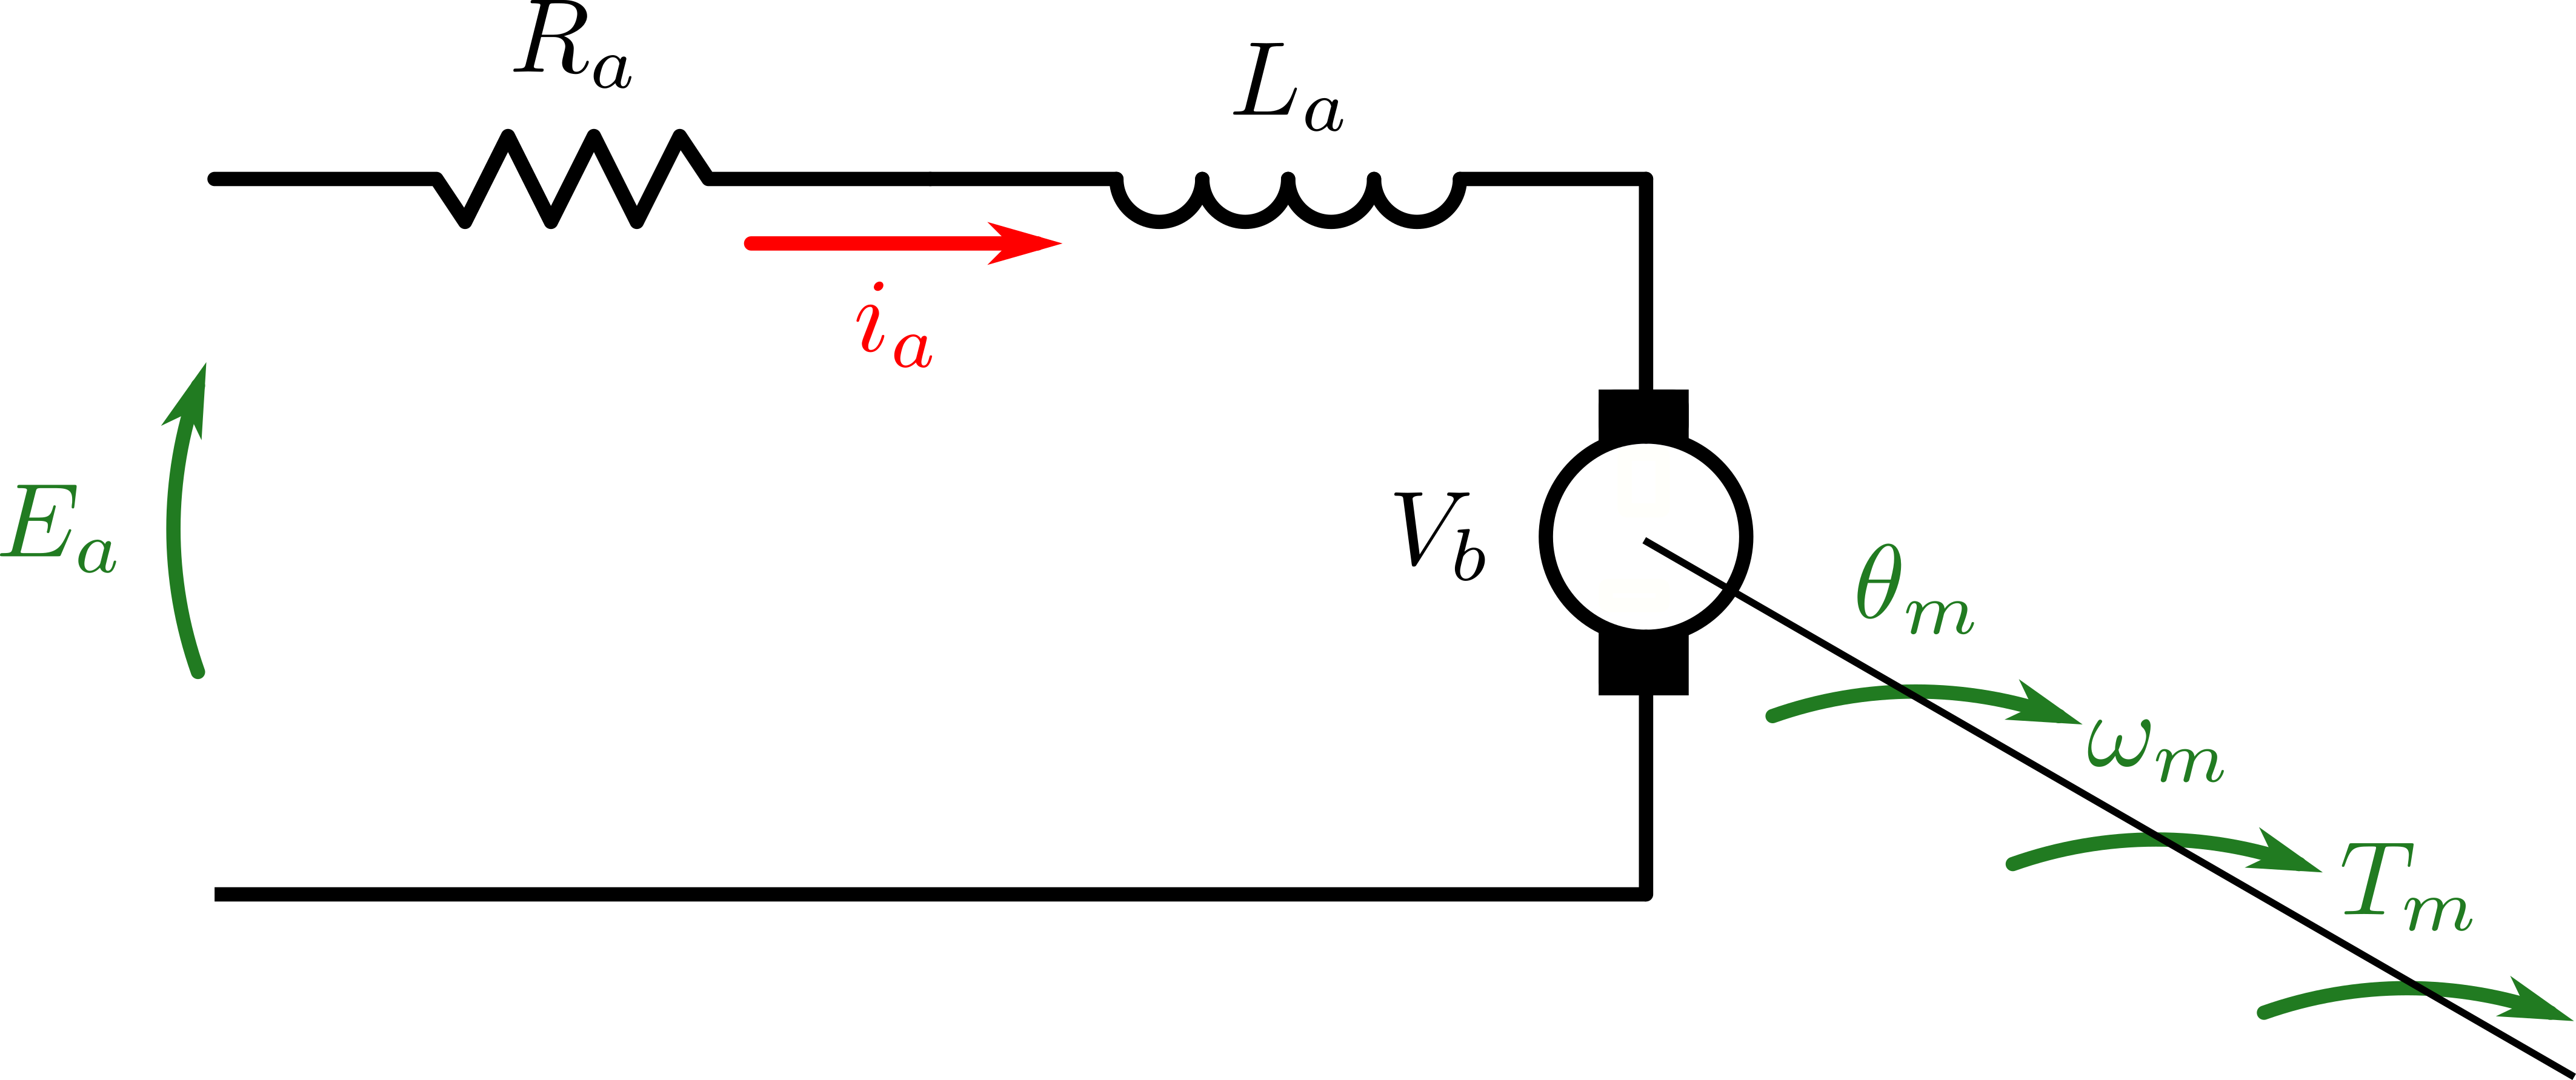
\includegraphics[width=0.5\linewidth]{../Images/ModeloMotor.png}
\end{figure}

Las ecuaciones que caracterizan al sistema son:

\[
\left\lbrace
\begin{array}{ll}
E_a = R_a \cdot i_a + L_a \cdot \dot{i_a} + V_b \\
V_b = K_b \cdot \omega_m = K_b \cdot \dot{\theta_m} \\
T_m = J_m \cdot \ddot{\theta_m} + B_m \cdot \dot{\theta_m}
\end{array}
\right.
\]

De las cuales se puede obtener las funciones de transferencia de $\theta_m$ y $\omega_m$ respecto a la tensión de alimentación $E_a$. Considerando que para continua (o muy baja frecuencia) no afecta la inductancia $L_a$, se obtiene:

\[
\frac{\omega_m}{E_a} = \frac{\frac{K_t}{R_a \cdot J_m}}{S + \frac{B_m}{J_m} + \frac{K_t \cdot K_b}{R_a \cdot J_m}}
\]

\[
\frac{\theta_m}{E_a} = \frac{\frac{K_t}{R_a \cdot J_m}}{S \cdot (S + \frac{B_m}{J_m} + \frac{K_t \cdot K_b}{R_a \cdot J_m})}
\]

De donde se puede construir el diagrama en bloques:

\begin{figure}[H]
\centering
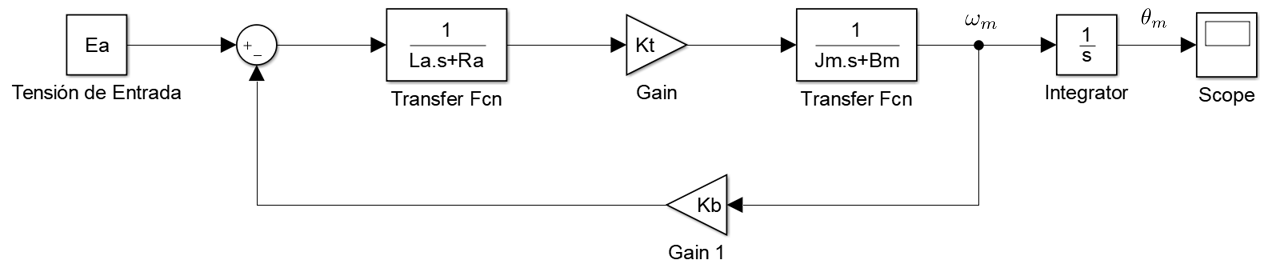
\includegraphics[width=1\linewidth]{../Images/DiagramaSimple.png}
\end{figure}


LO QUE VA ABAJO AL FINAL NO LO PONGO, SE USO EL METODO QUE DICE LA FILMINA DE CALCULO EMPIRICO ANULANDO UNA Y AJUSTANDO HASTA OSCILACION, Y DESPUES AJUSTAR LA OTRA. EDITAR EL CODIGO PARA QUE NO PAREZCA IGUAL
Se toman como variables de estado a $\theta_m$ y a $\omega_m$, armando las ecuaciones de estado:

\[
\left\lbrace
\begin{array}{ll}
\dot{\theta_m} = \omega_m \\
\dot{\omega_m} = E_a \cdot \frac{K_t}{R_a \cdot J_m} - \omega_m \cdot ( \frac{B_m}{J_m} + \frac{K_t \cdot K_b}{R_a \cdot J_m} )
\end{array}
\right.
\]

Por lo que el espacio de estados matricial resulta:

\[
\begin{bmatrix}
\dot{\theta_m} \\
\dot{\omega_m} 
\end{bmatrix}
=
\begin{bmatrix}
0 & 1 \\
0 & \left( \frac{B_m}{J_m} + \frac{K_t \cdot K_b}{R_a \cdot J_m} \right) 
\end{bmatrix}
\cdot
\begin{bmatrix}
\theta_m \\
\omega_m 
\end{bmatrix}
+
\begin{bmatrix}
0 \\
\frac{K_t}{R_a \cdot J_m}
\end{bmatrix}
\cdot
\begin{bmatrix}
E_a
\end{bmatrix}
\]

\section{Driver para señales}

Para realizar la realimentación lineal de estados, se implementó mediante un software en Arduino. Por ello se debieron adaptar las señales de los sensores, para lo cual se realizó una placa adicional como driver.

\subsection{Motor - Puente H}
El motor acepta como máxima tensión de alimentación 6V, por lo que alimentando a la placa con $\pm 10$V, se toman los +10V y se pasan por un regulador LM7806, y de ahí se toma la alimentación para el puente H (para el control del motor):

\begin{figure}[H]
\centering
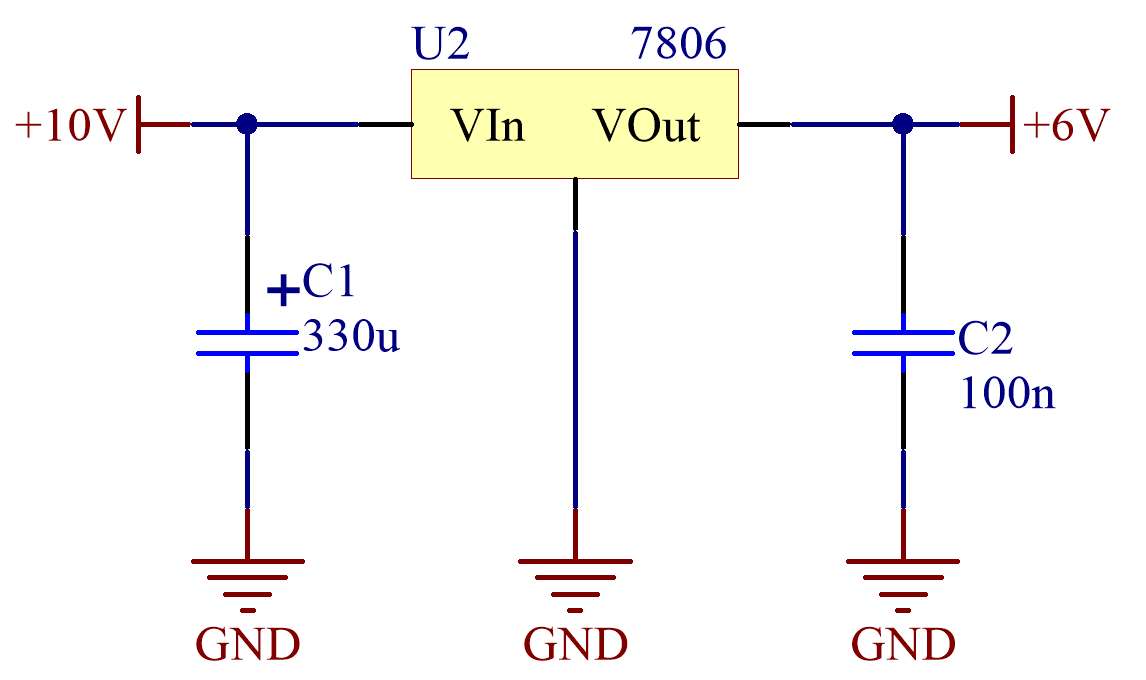
\includegraphics[width=0.6\linewidth]{../Images/Regulador.png}
\end{figure}

\subsection{Potenciómetro (Posición)}

Para el potenciómetro que permite medir la posición angular del motor, se lo alimenta con 6V y se conecta la salida a una de las entradas analógicas de Arduino (A1):

\begin{figure}[H]
\centering
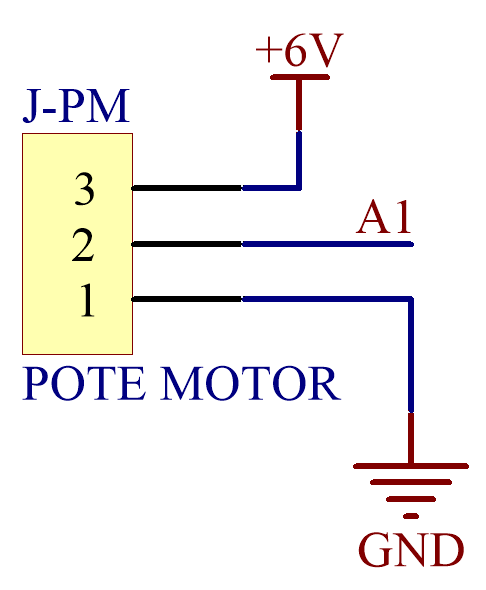
\includegraphics[width=0.2\linewidth]{../Images/PoteMotor.png}
\end{figure}

\subsection{Tacómetro (Velocidad)}
Para adaptar la señal del tacómetro, dado que provee valores entre -5V y +5V, se implementó con un amplificador operacional una función lineal, tal que la salida se mapee al intervalo de 0V a 5V (que es el rango admitido por el Arduino).\par

\begin{figure}[H]
\centering
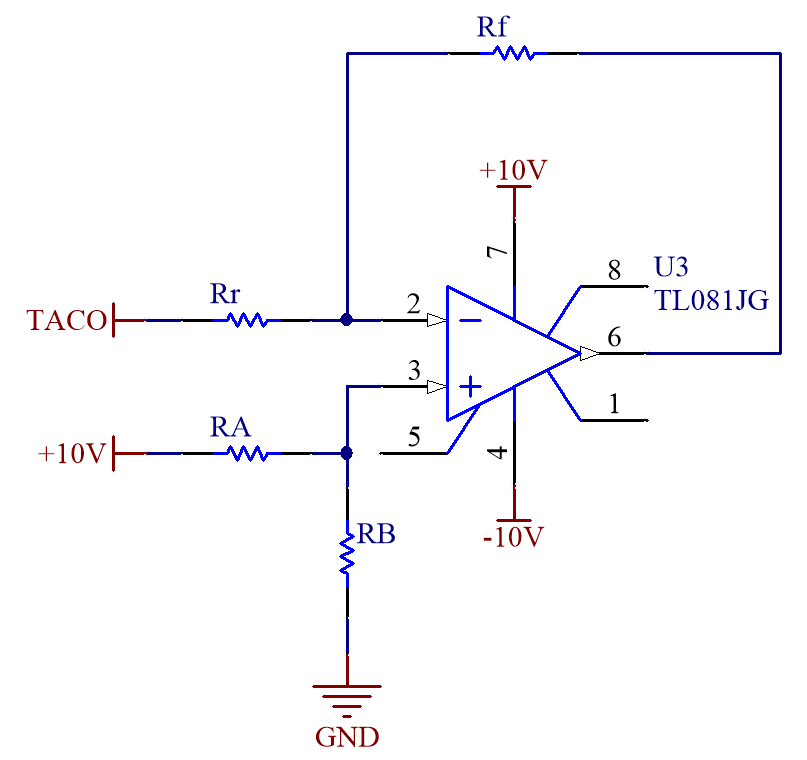
\includegraphics[width=0.45\linewidth]{../Images/ModeloFuncion.png}
\end{figure}

Considerando la transferencia de un amplificador inversor:

\[
A_V = - \frac{R_f}{R_r}
\]

El rango total inicial es de 20V, y el buscado es de 5V, por lo que el factor de escala es 4. De esta forma se toma $R_f = 1K$ y $R_r = 3K9 + 100$ (desdoblando esta última en dos resistencias en serie). Para el offset, se considera el divisor resistivo y la ganancia de un amplificador no inversor, tal que:

\[
10V \cdot \frac{R_B}{R_A + R_B} \cdot \left(1 + \frac{1}{4}\right) = 2.5V
\]

De esta forma el divisor resistivo resulta de $\frac{1}{5}$, por lo que se toma $R_B = 1K$ y $R_A = 3K9 + 100$ (desdoblando esta última en dos resistencias en serie). Finalmente, el circuito resultante es el siguiente:

\begin{figure}[H]
\centering
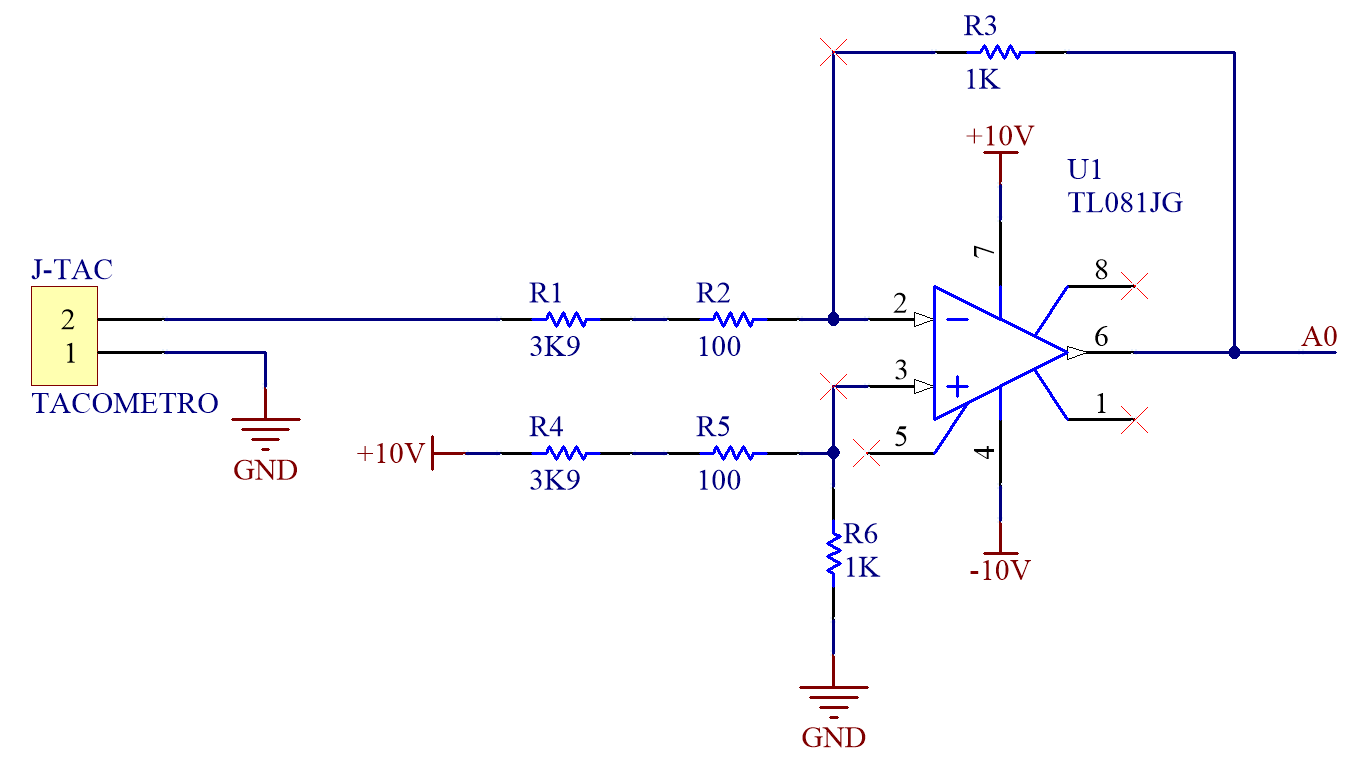
\includegraphics[width=0.6\linewidth]{../Images/FuncionOpamp.png}
\end{figure}

\subsection{Señal de control por Potenciómetro}

Para el potenciómetro de señal de control manual, utilizando la misma alimentación de 6V saliente del regulador, se le colocó una resistencia en serie tal que la máxima salida sea de 5V:

\begin{figure}[H]
\centering
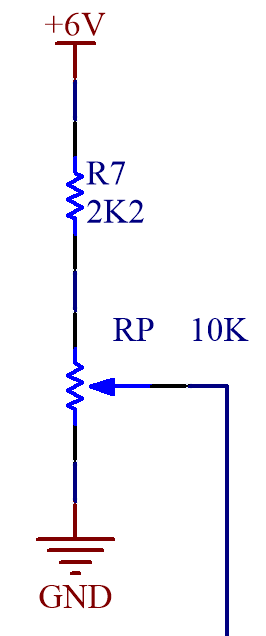
\includegraphics[width=0.1\linewidth]{../Images/PoteManual.png}
\end{figure}

\section{Simulación y Mediciones}



\subsection{Entrada por señal}

\subsubsection{Rectangular}

\subsubsection{Triangular}

\subsubsection{Senoidal}


\subsection{Entrada por potenciómetro}

\end{document}
